%%%%%%%%%%%%%%%%%%%%%%%%%%%%%%%%%%%%%%%%%%%%%%%%%%%%%%%%%
%                 File: UV1310cdc.tex               	%
%                  Date: 10 Oct, 2015                	%
%                                                    	%
%   For submission to a OFC      						%
%                                                     	%
%   Technical paper about the results obtained with   	%
%   professor Wei Shi with tunable cascaded				%
%	contra-directional coupler				      		%
%	+ theorical analysis								%
%%%%%%%%%%%%%%%%%%%%%%%%%%%%%%%%%%%%%%%%%%%%%%%%%%%%%%%%%



\documentclass[letterpaper,10pt]{article}
\usepackage{osameet2}

\usepackage[utf8]{inputenc} %encoding of the input(this text file)
\usepackage[T1]{fontenc} 	%uses the right font encoding
\usepackage{lmodern,textcomp}		%makes font work for fontenc
\usepackage[french,english]{babel} %multiple languages
\selectlanguage{english}	%can switch to french later using this

\usepackage{ulem}
\usepackage{amsmath,amssymb}

\usepackage{graphicx,epsfig,epstopdf}

\usepackage{xcolor}
\newcommand\todo[1]{\textcolor{red}{#1}}
\renewcommand\todo[1]{}  %activate to get rid of comments

\begin{document}
	
	\title{O-band Silicon Photonic Bragg-Grating Multiplexers using UV Lithography}
	
	\author{Jonathan St-Yves, Sophie Larochelle, and Wei Shi$^*$}
	\address{Centre d'optique, photonique et laser (COPL) and Département de génie électrique, Université Laval, 2375 rue de la Terrasse, Québec (Québec), Canada, G1V 0A6}
	%\email{jonathan.st-yves.1@ulaval.ca}
	\email{$^*$wei.shi@gel.ulaval.ca}
	
	\begin{abstract}
		We demonstrate the first Bragg-grating-based 4-channel O-band (de-)multiplexer fabricated using 193nm lithography on submicron-SOI with small features below 140nm.
	\end{abstract}
	
	\ocis{ (130.7408) Wavelength filtering devices; (350.2770) Gratings; (130.3120)   Integrated optics devices}
	
	\maketitle
	
	\section{Introduction}
	Integrated optical filters are key components for next-generation communications applications enabling cloud services, video streaming and other data-heavy applications. Applying wavelength division multiplexing (WDM) in data centers allows fibers to transport more information, which requires high performance, low-cost filters and multiplexers that work in the O-band near 1310 nm, where the chromatic dispersion in conventional fibers is minimal. 
	
	Integrated WDM on the submicron silicon-on-insulator (SOI) platform can be achieved using lattice filters\cite{horst2013cascaded} or arrayed waveguides \cite{okamoto2013fabrication}, though these methods use a large footprint and have limited free-spectral ranges (FSRs). Others possible approaches include Bragg gratings\cite{simard2012apodized} and micro-ring filters\cite{xu2006cascaded}. However, conventional Bragg gratings work in the reflection mode, requiring circulators or interferometers for wavelength multiplexing. Micro-ring filters also suffer from small FSRs. In addition, most existing SOI filters have been in the C-band near 1550 nm, while O-band may be more important for short-reach applications such as data centers.
	
	Contra-directional couplers (contra-DCs) are Bragg-grating assisted add-drop filters that offer large bandwidth, flat-top response, compact footprint, and high sidelobes suppression \cite{shi2013siliconContraDC}. But they require small features (e.g., coupler gap and corrugations) for gratings, which limits the performance when fabricated using deep-ultraviolet lithography for mass production \cite{shi2013siliconContraDC}\cite{shi2013coupler}. This issue is compounded when designing a device for the O-band as the small wavelength size requires a proportionally smaller grating step.
	
	In this paper, we propose a novel contra-DC geometry in a rib waveguide to increase the mode coupling and thus relax the request for small features. The design is implemented using a CMOS-compatible process with 193 nm lithography and a phase-shift mask.  We present results for a 4 channel mu/demultiplexer in the O-band with high sidelobes suppression.
	
	
	\section{Device}
	\subsection{Design} 
	\begin{figure}[htbp]
		\centering
		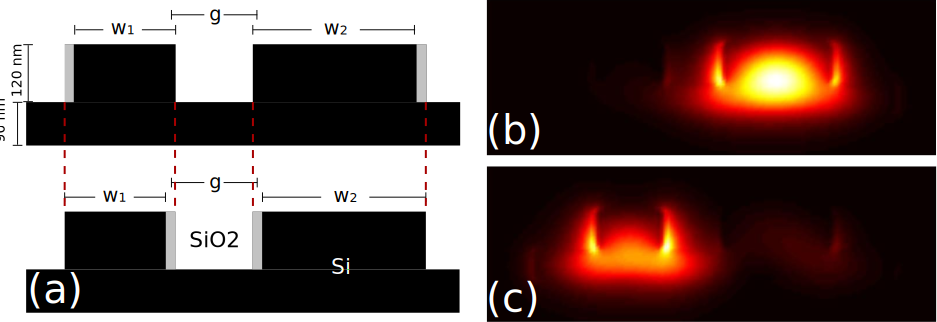
\includegraphics[width=.60\columnwidth]{CrossSection3}
		\caption{ a)Schematics of the cross-section over a period when close (top) and far (bottom): $w_1$ and $w_2$ are the waveguide widths, and $g$ the average gap. b) and c) Intensity distribution of the first and second supermodes. }
		\label{fig:Device}
	\end{figure}
	
	The contra-DC filters and cascaded multiplexers are designed for the standard 220-nm SOI wafer. Each contra-DC consists of two waveguides in close proximity, with a periodic dielectric perturbations, i.e., Bragg gratings, in the gap region. This introduces a wavelength-selective, contra-directional coupling at  $\lambda_\text{c} = \Lambda (n_\text{1}+n_\text{2})$, where $\Lambda$ is the grating pitch, and $n_\text{1}$ and $n_\text{2}$ are the effective refractive indices of the first-order and second-order eigenmodes in the coupler. 
	The waveguides are highly asymmetric to suppress the co-directional coupling that would occur with two identical waveguides.
	
	Figure \ref{fig:Device} shows the  cross-section of the proposed contra-DC. We observe that the mode confinement is relatively weak due to the small waveguide widths (220 nm and 360 nm) and the existence of the slab in between. Therefore, there is a much stronger mode overlap with the grating corrugations, compared to the previously demonstrated device in strip waveguides. This allows us to design contra-DCs with a stronger coupling which enables a large bandwidth with a relatively large feature size. The contra-DCs are apodized to reduce side-lobes using a gaussian profile in the coupling with an apodization index $a=10$, following the method described in \cite{shi2013siliconContraDC}.
	
	\subsection{Fabrication}
	The fabrication was performed using a CMOS compatible silicon photonic process with deep UV (193 nm) lithography, offered by IME, Singapore. It uses a phase shift mask which allows high precision for small features such as grating corrugations. 
	
	Figure \ref{fig:litho} b) shows the SEM image of a fabricated device. We can see clearly see the grating corrugations, even though the square shaped corrugations in the layout design are smoothed in the lithography as expected. Corrugations with a small period of 260 nm and gaps under 140 nm are resolved. However, the width of the waveguide in this strong corrugation region is uneven due to the approximation effect on the internal sidewall compared to the external. This also results in a strong change of index along the propagation direction and thus distortion of the apodization profile, as seen in the measured spectra discussed below.
	
	\begin{figure}[htbp]
		\centering
		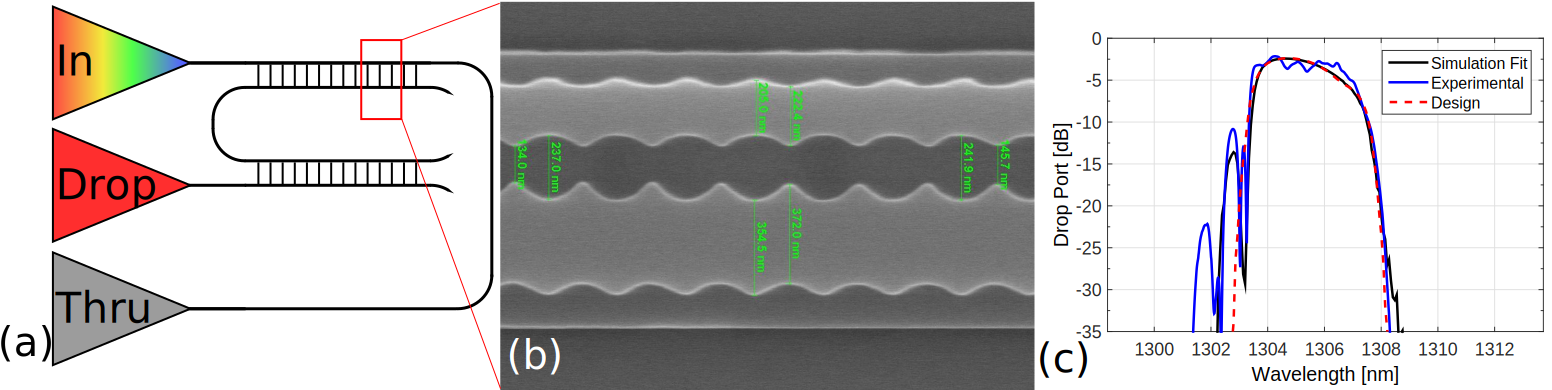
\includegraphics[width=.99\columnwidth]{SingleFilterFig}
		\caption{ a) Schematic of a dual-stage single-channel contra-DC. b)SEM showing that the waveguide widths vary in the close and far regions. c) Simulated and measured spectral response of the dual-stage contra-DC, with fiber-to-chip response subtracted.}
		\label{fig:litho}
	\end{figure}
	
	\subsection{Experimental results}
	Figure \ref{fig:litho} c) shows the spectral response of a dual stage filter. The insertion loss is 2.5 dB, the bandwidth covers 370 GHz and the sidelobe suppression is 8 dB. This relatively weak sidelobes suppression is explained by the fact that strong corrugations are uneven on both sides, causing the effective index to be higher in the strong coupling regions than in the low coupling regions, which creates coupling dependent chirp; an different wavelength Bragg-condition along the grating. 
	
	This coupling dependent chirp is considered in the simulation fit, which agrees with experimental results. With this information, we will be able to bias future devices to cancel this effect and create even gratings despite lithography distortion.
	
	%\subsection{WDM performance}
	\begin{figure}[htbp]
		\centering
		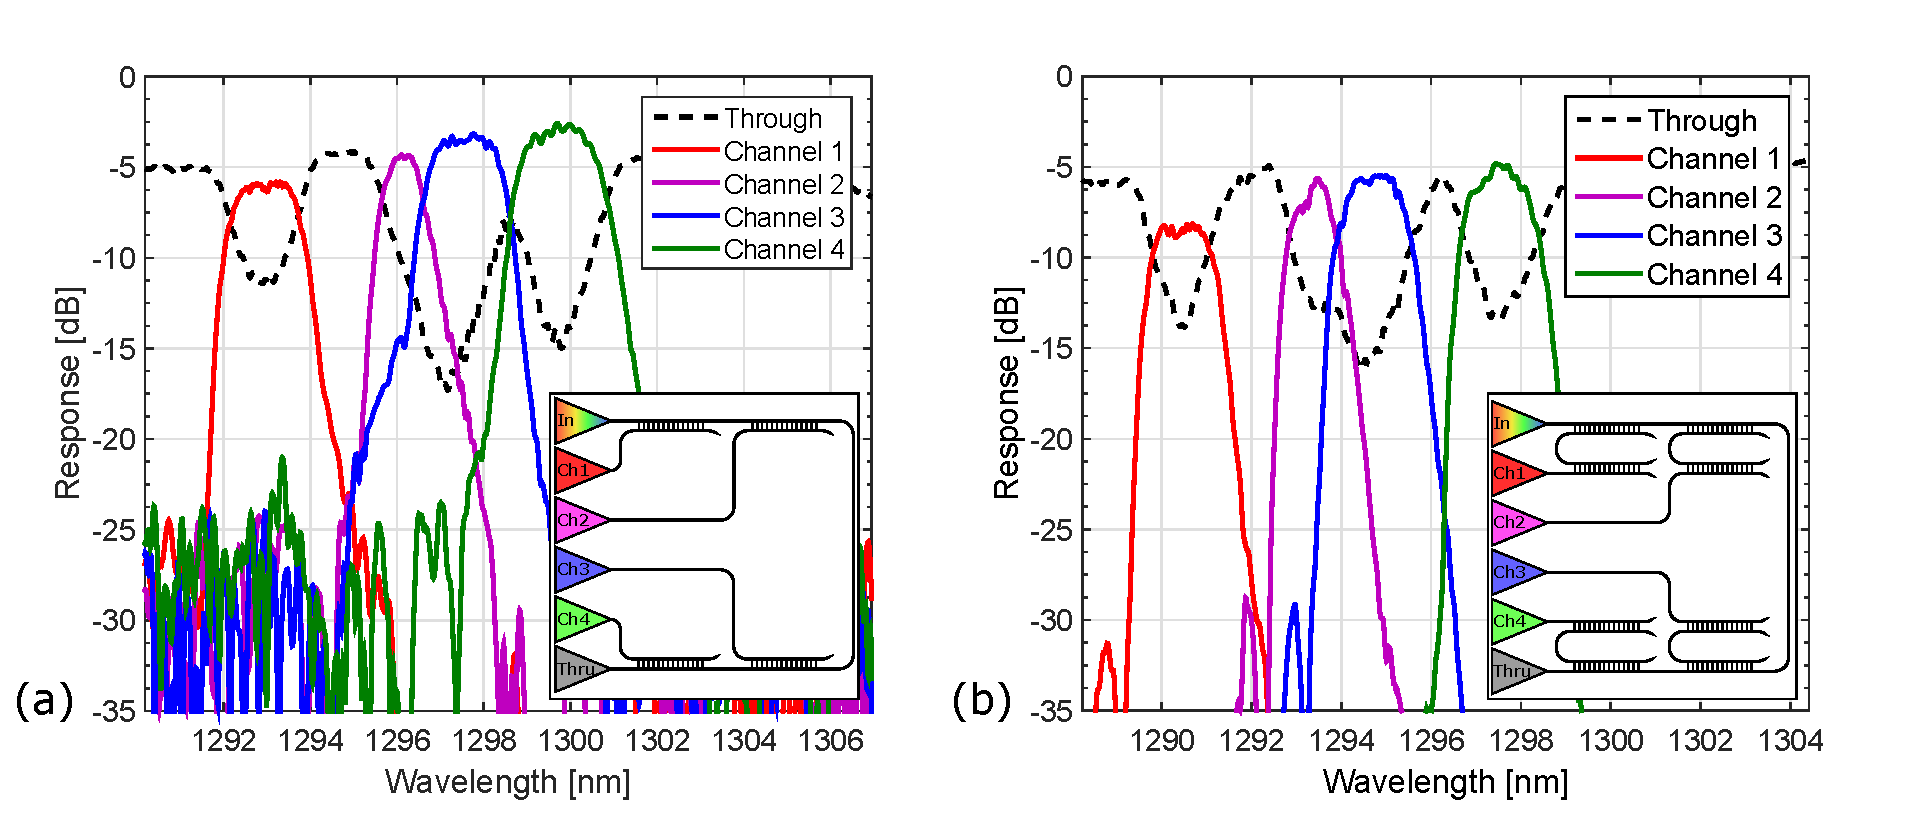
\includegraphics[width=.8\columnwidth]{WDM}
		\caption{a) Measured spectra of a single-stage contra-DC WDM. ~~~~~~b) Dual-stage WDM.}
		\label{fig:WDM}
	\end{figure}
	
	Figure \ref{fig:WDM} shows the performance of four serial cascaded filters for a 4-channel wavelength multiplexer or demultiplexer, for single stage and dual stage filtering. The contra-DCs in different channels have slightly different pitch ($\Lambda$) for specific wavelengths. The channels are dropped in reverse order such that channel 3 has precedence over channel 2. This explains why smaller channel numbers experience a higher loss, they have a longer optical path through more devices. An obvious problem is that the second channel is smaller and offset. This is a systematic glitch in all the devices we measured, caused by the fact that channel 2 has an even grating pitch of 260 nm and that the grid resolution of the fabrication is 1 nm, causing it to snap differently to the grid then the other devices. This causes its effective index and central wavelength to be slightly higher.
	
	
	\section{Conclusion}
	In summery, we demonstrated, for the first time, Bragg-grating-based multiplexers in the O-band on submicron SOI using UV lithography. This technology is a key enabler for low cost and flexible WDM in data centers. 
	The prototype presented gives the community critical information about the possible issues when using UV lithography for small features and how to consider them for future designs.
	
	\section*{Acknowledgments}
	We acknowledge CMC Microsystems for the  software and the fabrication subsidy. The authors acknowledge the Natural Sciences and Engineering Research Council of Canada for funding this research. This work is part of the SPEED research project funded by NSERC, PROMPT, and TeraXion.
	
	\bibliographystyle{osajnl}
	\bibliography{bibli}
	
\end{document}